\documentclass[utf8,usehyperref,12pt]{G7-32}
\input glyphtounicode.tex                   % Нужно для
\pdfgentounicode=1                          % поиска по pdf в кириллице
\usepackage[T2A]{fontenc}
\usepackage{pscyr}
\usepackage[utf8]{inputenc}                 % ваша любимая кодировка здесь
\usepackage[english,russian]{babel}         % это необходимо для включения переносов
\usepackage{float}
\usepackage[pdftex]{graphicx}
\usepackage{array}
\usepackage{mversion}                       % Версионирование
\TableInChaper                              % таблицы будут нумероваться в пределах раздела
\PicInChaper                                % рисунки будут нумероваться в пределах раздела
\setlength\GostItemGap{2mm}                 % для красоты можно менять от 0мм
\sloppy                                     % переносы

\newcounter{MinoreCounter}                  % Новый счетчик минорных версий
\setcounter{MinoreCounter}{1}               % Текущая минорная версия

\renewcommand{\theequation}{(\arabic{chapter}.\arabic{equation})}   % Формат нумерации формул "Глава.номер"
\renewcommand{\version}{\versionnumber.\theMinoreCounter.\thebuildcounter} % Формат версии

\makeatletter
\@addtoreset{equation}{chapter}             % Счетчик формул
\makeatother

\setcounter{page}{2}                        % Начало нумерации страниц
\setVersion{0}                              % Текущая мажорная версия
\increaseBuild                              % Увеличивать номер сборки при каждой компиляции
%<------------- НАЧАЛО ДОКУМЕНТА ---------------------------


\begin{document}
\tableofcontents

\begin{center}
Текущая версия документа: \version~от \today 
\end{center}

\chapter{Введение}
Это пример оформления документации на программу имитации приемо-передающей системы в рамках второго семестра курса <<Радиотехника>>, оформленная в среде \LaTeX{}

\chapter{Описание программы}
Тут располагается описание и назначение программы. В состав демонстрационной программы входят модули \verb\Sender.py\, \verb\Receiver.py\, \verb\Plot.py\, \verb\Form.py\
\section{Описание модуля Sender}
Модуль \verb\Sender.py\ состоит из класса \verb\Sender\. Класс имитирует передатчик и реализует атрибуты-методы,
которые существуют в реальной системе. Конструктор класса принимает следующие параметры:

\begin{itemize}
\item \verb\FD_\ -- Частота дискретизации аналогового несущего сигнала
\item \verb\FDD_\ -- Частота дискретизации цифрового исходного сигнала
\item \verb\FC_\ -- Частота несущей
\item \verb\N_\ -- Количество передающихся символов
\item \verb\SPEED_\ -- Символьная скорость (частота символов)
\item \verb\A_NOISE_\ -- Амплитуда шума
\item \verb\A_SIGNAL_\ -- Амплитуда сигнала
\end{itemize}

Пример использования в коде:
\begin{verbatim}
self.sender_obj = Sender(FD,
                         FDD,
                         FC,
                         N,
                         SPEED,
                         A_NOISE,
                         A_SIGNAL)
\end{verbatim}

\chapter{Скриншоты работы программы}

\begin{figure}[H]
\begin{center}
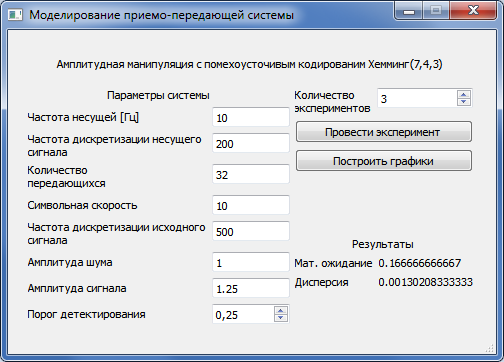
\includegraphics[scale=1]{Image/1.png}
\caption{Пример работы программы}
\end{center}
\end{figure}

\begin{figure}[H]
\begin{center}
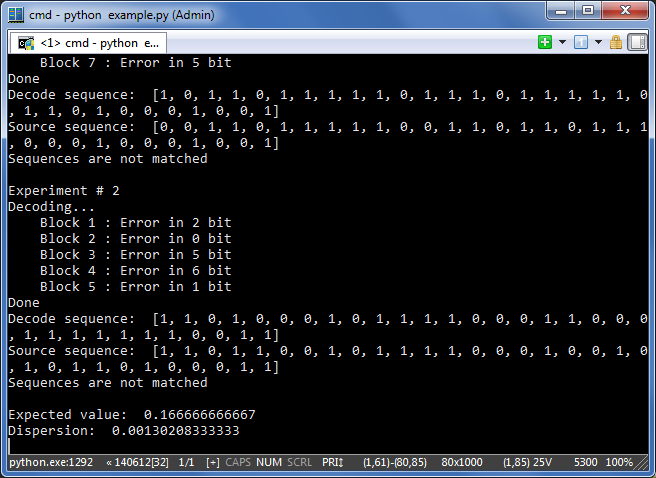
\includegraphics[scale=0.8]{Image/2.png}
\caption{Пример вывода в консоль}
\end{center}
\end{figure}

\begin{figure}[H]
\begin{center}
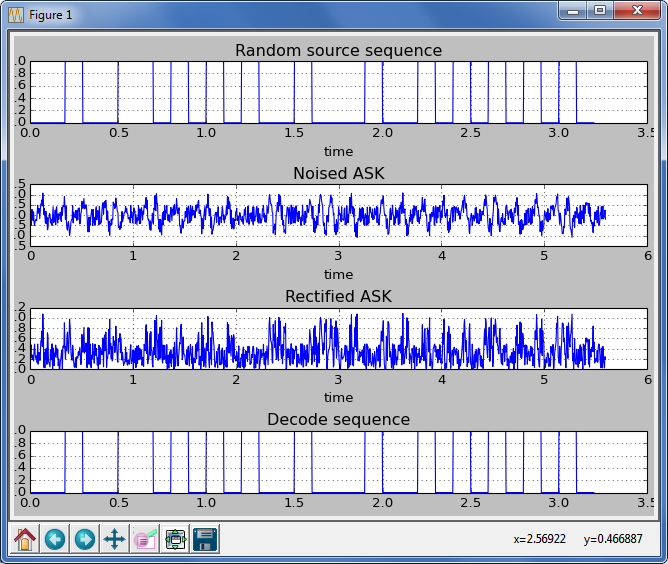
\includegraphics[scale=0.8]{Image/3.png}
\caption{Пример построения графиков}
\end{center}
\end{figure}
\end{document}